% Preamble templated from Mihir-Divyansh/Course-Setup
%iffalse
\let\negmedspace\undefined
\let\negthickspace\undefined
\documentclass[journal,12pt,onecolumn]{IEEEtran}
\usepackage{cite}
\usepackage{amsmath,amssymb,amsfonts,amsthm}
\usepackage{algorithmic}
\usepackage{graphicx}
\usepackage{textcomp}
\usepackage{xcolor}
\usepackage{txfonts}
\usepackage{listings}
\usepackage{enumitem}
\usepackage{mathtools}
\usepackage{gensymb}
\usepackage{comment}
\usepackage[breaklinks=true]{hyperref}
\usepackage{tkz-euclide}
\usepackage{listings}
\usepackage{gvv}
%\def\inputGnumericTable{}
\usepackage[latin1]{inputenc}
\usepackage{color}
\usepackage{array}
\usepackage{longtable}
\usepackage{calc}
\usepackage{multirow}
\usepackage{hhline}
\usepackage{ifthen}
\usepackage{lscape}
\usepackage{tabularx}
\usepackage{array}
\usepackage{float}
\usepackage{caption}
\usepackage{multicol}
\usepackage{tfrupee}

\newtheorem{theorem}{Theorem}[section]
\newtheorem{problem}{Problem}
\newtheorem{proposition}{Proposition}[section]
\newtheorem{lemma}{Lemma}[section]
\newtheorem{corollary}[theorem]{Corollary}
\newtheorem{example}{Example}[section]
\newtheorem{definition}[problem]{Definition}
\newcommand{\BEQA}{\begin{eqnarray}}
\newcommand{\EEQA}{\end{eqnarray}}
\newcommand{\define}{\stackrel{\triangle}{=}}
\theoremstyle{remark}
\newtheorem{rem}{Remark}

% Marks the beginning of the document
\begin{document}
\bibliographystyle{IEEEtran}
\vspace{3cm}

\title{Assignment 4: GATE 2022 PH: Physics}
\author{EE25BTECH11055 - Subhodeep Chakraborty}
\maketitle
\hrulefill
\bigskip

\renewcommand{\thefigure}{\theenumi}
\renewcommand{\thetable}{\theenumi}


\begin{enumerate}

\item
You should \rule{1cm}{0.4pt} when to say \rule{1cm}{0.4pt}.
\begin{enumerate}
    \item no/no
    \item no/know
    \item know / know
    \item know/no
\end{enumerate}


\item
Two straight lines pass through the origin $(x_{0},y_{0})=(0,0)$. One of them passes through the point $(x_{1},y_{1})=(1,3)$ and the other passes through the point $(x_{2},y_{2})=(1,2)$. What is the area enclosed between the straight lines in the interval [0, 1] on the x-axis?
\begin{enumerate}
    \item 0.5
    \item 1.0
    \item 1.5
    \item 2.0
\end{enumerate}


\item
If $p:q=1:2$, $q:r=4:3$, $r:s=4:5$ and u is 50\% more than s, what is the ratio p: u?
\begin{enumerate}
    \item 2:15
    \item 16:15
    \item 1:5
    \item 16:45
\end{enumerate}


\item
Given the statements:
\begin{itemize}
    \item P is the sister of Q.
    \item Q is the husband of R.
    \item R is the mother of S.
    \item T is the husband of P.
\end{itemize}
Based on the above information, T is \rule{1cm}{0.4pt} of S.
\begin{enumerate}
    \item the grandfather
    \item an uncle
    \item the father
    \item a brother
\end{enumerate}


\item
In the following \figref{fig:5}, the point R is the center of the circle. The lines PQ and ZV are tangential to the circle. The relation among the areas of the squares, PXWR, RUVZ and SPQT is
\begin{center}
    \begin{figure}[H] \caption{} \label{fig:5}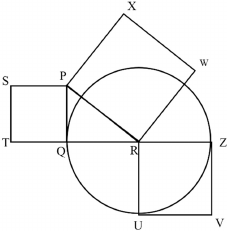
\includegraphics{figs/5.png}\end{figure}%[width=0.4\textwidth]{p4_diagram.png}
\end{center}
\begin{enumerate}
    \item Area of SPQT = Area of RUVZ = Area of PXWR
    \item Area of SPQT = Area of PXWR - Area of RUVZ
    \item Area of PXWR = Area of SPQT - Area of RUVZ
    \item Area of PXWR = Area of RUVZ - Area of SPQT
\end{enumerate}


\item
Healthy eating is a critical component of healthy aging. When should one start eating healthy? It turns out that it is never too early. For example, babies who start eating healthy in the first year are more likely to have better overall health as they get older.
Which one of the following is the CORRECT logical inference based on the information in the above passage?
\begin{enumerate}
    \item Healthy eating is important for those with good health conditions, but not for others
    \item Eating healthy can be started at any age, earlier the better
    \item Eating healthy and better overall health are more correlated at a young age, but not older age
    \item Healthy eating is more important for adults than kids
\end{enumerate}


\item
P invested \rupee 5000 per month for 6 months of a year and Q invested \rupee x per month for 8 months of the year in a partnership business. The profit is shared in proportion to the total investment made in that year. If at the end of that investment year, Q receives $\frac{4}{9}$ of the total profit, what is the value of x (in \rupee)?
\begin{enumerate}
    \item 2500
    \item 3000
    \item 4687
    \item 8437
\end{enumerate}


\item
The frequency chart in \figref{fig:8} shows the frequency distribution of marks obtained by a set of students in an exam.
\begin{center}
    \begin{figure}[H] \caption{} \label{fig:8}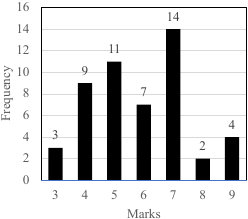
\includegraphics{figs/8.png}\end{figure}%[width=0.6\textwidth]{p7_diagram.png}
\end{center}
From the data presented above, which one of the following is CORRECT?
\begin{enumerate}
    \item mean \textgreater mode \textgreater median
    \item mode \textgreater median \textgreater mean
    \item mode \textgreater mean \textgreater median
    \item median \textgreater mode \textgreater mean
\end{enumerate}


\item
In the square grid shown in \figref{fig:9}, a person standing at P2 position is required to move to P5 position. The only movement allowed for a step involves, "two moves along one direction followed by one move in a perpendicular direction". The permissible directions for movement are shown as dotted arrows in the right. For example, a person at a given position Y can move only to the positions marked X on the right. Without occupying any of the shaded squares at the end of each step, the minimum number of steps required to go from P2 to P5 is
\begin{center}
    \begin{figure}[H] \caption{} \label{fig:9}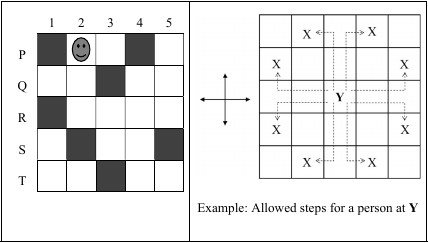
\includegraphics{figs/9.png}\end{figure}%[width=0.7\textwidth]{p8_diagram.png}
\end{center}
\begin{enumerate}
    \item 4
    \item 5
    \item 6
    \item 7
\end{enumerate}


\item
Consider a cube made by folding a single sheet of paper of appropriate shape. The interior faces of the cube are all blank. However, the exterior faces that are not visible in the above view may not be blank. Which one of the following represents a possible unfolding of the cube?
% Placeholder for diagram from page 9
\begin{center}
    \begin{figure}[H] \caption*{} \label{fig:10}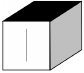
\includegraphics{figs/10.png}\end{figure}%[width=0.8\textwidth]{p9_diagram.png}
\end{center}
\begin{enumerate}
 \item \begin{figure}[H] \caption*{} \label{fig:10a}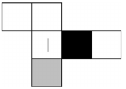
\includegraphics{figs/10a.png}\end{figure}
 \item \begin{figure}[H] \caption*{} \label{fig:10b}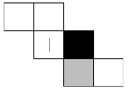
\includegraphics{figs/10b.png}\end{figure}
 \item \begin{figure}[H] \caption*{} \label{fig:10c}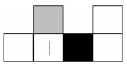
\includegraphics{figs/10c.png}\end{figure}
 \item \begin{figure}[H] \caption*{} \label{fig:10d}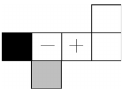
\includegraphics{figs/10d.png}\end{figure}
\end{enumerate}

\newpage

\item
For the Op-Amp circuit shown in \figref{fig:11}, choose the correct output waveform corresponding to the input $V_{in} = 1.5 \sin 20\pi t$ (in Volts). The saturation voltage for this circuit is $V_{sat} = \pm 10$ V.
\begin{center}
    \begin{figure}[H] \caption{} \label{fig:11}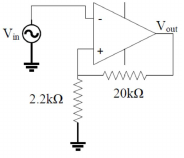
\includegraphics{figs/11.png}\end{figure}%[width=0.4\textwidth]{p10_circuit.png}
\end{center}
\begin{enumerate}
    \item \begin{figure}[H] \caption*{} \label{fig:11a}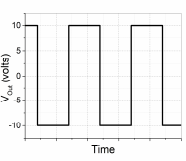
\includegraphics{figs/11a.png}\end{figure}%[width=0.4\textwidth]{p10_waveformA.png}
    \item \begin{figure}[H] \caption*{} \label{fig:11b}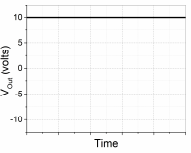
\includegraphics{figs/11b.png}\end{figure}%[width=0.4\textwidth]{p10_waveformB.png}
    \item \begin{figure}[H] \caption*{} \label{fig:11c}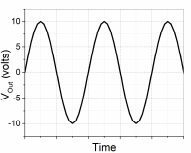
\includegraphics{figs/11c.png}\end{figure}%[width=0.4\textwidth]{p11_waveformC.png}
    \item \begin{figure}[H] \caption*{} \label{fig:11d}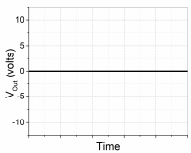
\includegraphics{figs/11d.png}\end{figure}%[width=0.4\textwidth]{p11_waveformD.png}
\end{enumerate}


\item
Match the order of $\beta$ – decays given in the left column to appropriate clause in the right column.
Here $X(I^\pi)$ and $Y(I^\pi)$ are nuclei with intrinsic spin $I$ and parity $\pi$.
\begin{center}
\begin{tabular}{ll}
    1. $X (\frac{1}{2}^+) \rightarrow Y (\frac{1}{2}^+)$ & i) First forbidden $\beta$-decay \\
    2. $X (\frac{1}{2}^-) \rightarrow Y (\frac{5}{2}^+)$ & ii) Second forbidden $\beta$-decay \\
    3. $X(3^+) \rightarrow Y(0^+)$ & iii) Third forbidden $\beta$-decay \\
    4. $X(4^-) \rightarrow Y(0^+)$ & iv) Allowed $\beta$-decay \\
\end{tabular}
\end{center}
\begin{enumerate}
    \item 1 - i, 2 - ii, 3 - iii, 4 - iv
    \item 1 - iv, 2 - i, 3 - ii, 4 - iii
    \item 1 - i, 2 - iii, 3 - ii, 4 - iv
    \item 1 - iv, 2 - ii, 3 - iii, 4 - i
\end{enumerate}


\item
What is the maximum number of free independent real parameters specifying an $n$-dimensional orthogonal matrix?
\begin{enumerate}
    \item $n(n - 2)$
    \item $(n - 1)^2$
    \item $\frac{n(n - 1)}{2}$
    \item $\frac{n(n + 1)}{2}$
\end{enumerate}


\item
An excited state of Ca atom is [Mg]3p$^5$4s$^2$3d$^1$. The spectroscopic terms corresponding to the total orbital angular momentum are
\begin{enumerate}
    \item S, P, and D
    \item P, D, and F
    \item P and D
    \item S and P
\end{enumerate}


\item
On the surface of a spherical shell enclosing a charge free region, the electrostatic potential values are as follows: One quarter of the area has potential $\phi_0$, another quarter has potential $2\phi_0$ and the rest has potential $4\phi_0$. The potential at the centre of the shell is (You can use a property of the solution of Laplace\textquotesingle s equation.)
\begin{enumerate}
    \item $\frac{11}{4}\phi_0$
    \item $\frac{11}{2}\phi_0$
    \item $\frac{7}{3}\phi_0$
    \item $\frac{7}{4}\phi_0$
\end{enumerate}


\item
A point charge q is performing simple harmonic oscillations of amplitude $A$ at angular frequency $\omega$. Using Larmor\textquotesingle s formula, the power radiated by the charge is proportional to
\begin{enumerate}
    \item $q \omega^2 A^2$
    \item $q \omega^4 A^2$
    \item $q^2 \omega^2 A^2$
    \item $q^2 \omega^4 A^2$
\end{enumerate}


\item
Which of the following relationship between the internal energy $U$ and the Helmholtz\textquotesingle s free energy $F$ is true?
\begin{enumerate}
    \item $U = -T^2 \left[ \frac{\partial (F/T)}{\partial T} \right]_V$
    \item $U = +T^2 \left[ \frac{\partial (F/T)}{\partial T} \right]_V$
    \item $U = +T \left[ \frac{\partial F}{\partial T} \right]_V$
    \item $U = -T \left[ \frac{\partial F}{\partial T} \right]_V$
\end{enumerate}


\item
If nucleons in a nucleus are considered to be confined in a three-dimensional cubical box, then the first four magic numbers are
\begin{enumerate}
    \item 2, 8, 20, 28
    \item 2, 8, 16, 24
    \item 2, 8, 14, 20
    \item 2, 10, 16, 28
\end{enumerate}


\item
Consider the ordinary differential equation \begin{align*}y'' - 2xy' + 4y = 0\end{align*} and its solution $y(x) = a + bx + cx^2$. Then
\begin{enumerate}
    \item $a = 0, c = -2b \neq 0$
    \item $c = -2a \neq 0, b = 0$
    \item $b = -2a \neq 0, c = 0$
    \item $c = 2a \neq 0, b = 0$
\end{enumerate}


\item
For an Op-Amp based negative feedback, non-inverting amplifier, which of the following statements are true?
\begin{enumerate}
    \item Closed loop gain \textless Open loop gain
    \item Closed loop bandwidth \textless Open loop bandwidth
    \item Closed loop input impedance \textgreater Open loop input impedance
    \item Closed loop output impedance \textless Open loop output impedance
\end{enumerate}


\item
From the pairs of operators given below, identify the ones which commute. Here $l$ and $j$ correspond to the orbital angular momentum and the total angular momentum, respectively.
\begin{enumerate}
    \item $l^2, j^2$
    \item $j^2, j_z$
    \item $j^2, l_z$
    \item $l_z, j_z$
\end{enumerate}


\item
For normal Zeeman lines observed $\|$ and $\perp$ to the magnetic field applied to an atom, which of the following statements are true?
\begin{enumerate}
    \item Only $\pi$-lines are observed $\|$ to the field
    \item $\sigma$-lines $\perp$ to the field are plane polarized
    \item $\pi$-lines $\perp$ to the field are plane polarized
    \item Only $\sigma$-lines are observed $\|$ to the field
\end{enumerate}


\item
Pauli spin matrices satisfy
\begin{enumerate}
    \item $\sigma_\alpha \sigma_\beta - \sigma_\beta \sigma_\alpha = i \epsilon_{\alpha\beta\gamma} \sigma_\gamma$
    \item $\sigma_\alpha \sigma_\beta - \sigma_\beta \sigma_\alpha = 2i \epsilon_{\alpha\beta\gamma} \sigma_\gamma$
    \item $\sigma_\alpha \sigma_\beta + \sigma_\beta \sigma_\alpha = \epsilon_{\alpha\beta\gamma} \sigma_\gamma$
    \item $\sigma_\alpha \sigma_\beta + \sigma_\beta \sigma_\alpha = 2\delta_{\alpha\beta}$
\end{enumerate}


\item
For the refractive index $n = n_r(\omega) + i n_{im}(\omega)$ of a material, which of the following statements are correct?
\begin{enumerate}
    \item $n_r$ can be obtained from $n_{im}$ and vice versa
    \item $n_{im}$ could be zero
    \item $n$ is an analytic function in the upper half of the complex $\omega$ plane
    \item $n$ is independent of $\omega$ for some materials
\end{enumerate}


\item
Complex function $f(z) = z + |z - a|^2$ ($a$ is a real number) is
\begin{enumerate}
    \item continuous at $(a, a)$
    \item complex-differentiable at $(a, a)$
    \item complex-differentiable at $(a, 0)$
    \item analytic at $(a, 0)$
\end{enumerate}


\item
If $g(k)$ is the Fourier transform of $f(x)$, then which of the following are true?
\begin{enumerate}
    \item $g(-k) = +g^*(k)$ implies $f(x)$ is real
    \item $g(-k) = -g^*(k)$ implies $f(x)$ is purely imaginary
    \item $g(-k) = +g^*(k)$ implies $f(x)$ is purely imaginary
    \item $g(-k) = -g^*(k)$ implies $f(x)$ is real
\end{enumerate}


\item
The ordinary differential equation \begin{align*}(1 - x^2)y'' - xy' + 9y = 0\end{align*} has a regular singularity at
\begin{enumerate}
    \item $-1$
    \item $0$
    \item $+1$
    \item no finite value of $x$
\end{enumerate}


\item
For a bipolar junction transistor, which of the following statements are true?
\begin{enumerate}
    \item Doping concentration of emitter region is more than that in collector and base region
    \item Only electrons participate in current conduction
    \item The current gain $\beta$ depends on temperature
    \item Collector current is less than the emitter current
\end{enumerate}


\item
Potassium metal has electron concentration of $1.4 \times 10^{28}$ m$^{-3}$ and the corresponding density of states at Fermi level is $6.2 \times 10^{46}$ Joule$^{-1}$ m$^{-3}$. If the Pauli paramagnetic susceptibility of Potassium is $n \times 10^{-k}$ in standard scientific form, then the value of k (an integer) is \rule{1cm}{0.4pt}. (Magnetic moment of electron is $9.3 \times 10^{-24}$ Joule T$^{-1}$; permeability of free space is $4\pi \times 10^{-7}$ T m A$^{-1}$)


\item
A power supply has internal resistance $R_S$ and open load voltage $V_S = 5$ V. When a load resistance $R_L$ is connected to the power supply, a voltage drop of $V_L = 4$ V is measured across the load. The value of $\frac{R_L}{R_S}$ is \rule{1cm}{0.4pt} (Round off to the nearest integer)


\item
Electric field is measured along the axis of a uniformly charged disc of radius 25 cm. At a distance $d$ from the centre, the field differs by 10\% from that of an infinite plane having the same charge density. The value of $d$ is \rule{1cm}{0.4pt} cm. (Round off to one decimal place)


\item
In a solid, a Raman line observed at 300 cm$^{-1}$ has intensity of Stokes line four times that of the anti-Stokes line. The temperature of the sample is \rule{1cm}{0.4pt} K. (Round off to the nearest integer) (1 cm$^{-1} \equiv 1.44$ K)


\item
An electromagnetic pulse has a pulse width of $10^{-3}$ s. The uncertainty in the momentum of the corresponding photon is of the order of $10^{-N}$ kg m s$^{-1}$, where $N$ is an integer. The value of $N$ is \rule{1cm}{0.4pt}. (speed of light = $3 \times 10^8$ m s$^{-1}$, $h = 6.6 \times 10^{-34}$ J s)


\item
The wavefunction of a particle in a one-dimensional infinite well of size $2a$ at a certain time is $\psi(x) = \frac{1}{\sqrt{6a}} \left[ \sqrt{2}\sin\left(\frac{\pi x}{a}\right) + \sqrt{3}\cos\left(\frac{\pi x}{2a}\right) + \cos\left(\frac{3\pi x}{2a}\right) \right]$. Probability of finding the particle in n = 2 state at that time is \rule{1cm}{0.4pt}\% (Round off to the nearest integer)


\item
A spectrometer is used to detect plasma oscillations in a sample. The spectrometer can work in the range of $3 \times 10^{12}$ rad s$^{-1}$ to $30 \times 10^{12}$ rad s$^{-1}$. The minimum carrier concentration that can be detected by using this spectrometer is $n \times 10^{21}$ m$^{-3}$. The value of $n$ is \rule{1cm}{0.4pt}. (Round off to two decimal places) (Charge of an electron = $-1.6 \times 10^{-19}$ C, mass of an electron = $9.1 \times 10^{-31}$ kg and $\epsilon_0 = 8.85 \times 10^{-12}$ C$^2$ N$^{-1}$ m$^{-2}$)


\item
Consider a non-interacting gas of spin 1 particles, each with magnetic moment $\mu$, placed in a weak magnetic field $B$, such that $\frac{\mu B}{k_B T} \ll 1$. The average magnetic moment of a particle is
\begin{enumerate}
    \item $\frac{2\mu}{3} \left( \frac{\mu B}{k_B T} \right)$
    \item $\frac{\mu}{2} \left( \frac{\mu B}{k_B T} \right)$
    \item $\frac{\mu}{3} \left( \frac{\mu B}{k_B T} \right)$
    \item $\frac{3\mu}{4} \left( \frac{\mu B}{k_B T} \right)$
\end{enumerate}


\item
Water at 300 K can be brought to 320 K using one of the following processes.
Process 1: Water is brought in equilibrium with a reservoir at 320 K directly.
Process 2: Water is first brought in equilibrium with a reservoir at 310 K and then with the reservoir at 320 K.
Process 3: Water is first brought in equilibrium with a reservoir at 350 K and then with the reservoir at 320 K.
The corresponding changes in the entropy of the universe for these processes are $\Delta S_1$, $\Delta S_2$ and $\Delta S_3$, respectively. Then
\begin{enumerate}
    \item $\Delta S_2 > \Delta S_1 > \Delta S_3$
    \item $\Delta S_3 > \Delta S_1 > \Delta S_2$
    \item $\Delta S_3 > \Delta S_2 > \Delta S_1$
    \item $\Delta S_1 > \Delta S_2 > \Delta S_3$
\end{enumerate}


\item
A student sets up Young\textquotesingle s double slit experiment with electrons of momentum $p$ incident normally on the slits of width w separated by distance $d$. In order to observe interference fringes on a screen at a distance $D$ from the slits, which of the following conditions should be satisfied?
\begin{enumerate}
    \item $\frac{\hbar}{p} > \frac{Dw}{d}$
    \item $\frac{\hbar}{p} > \frac{dw}{D}$
    \item $\frac{\hbar}{p} > \frac{d^2}{D}$
    \item $\frac{\hbar}{p} > \frac{d^2}{\sqrt{Dw}}$
\end{enumerate}


\item
Consider a particle in three different boxes of width $L$. The potential inside the boxes vary as shown in \figref{fig:39} with $V_0 \ll \frac{\hbar^2\pi^2}{2mL^2}$. The corresponding ground-state energies of the particle are $E_1$, $E_2$ and $E_3$, respectively. Then
% Placeholder for diagram from page 25
\begin{center}
    \begin{figure}[H] \caption{} \label{fig:39}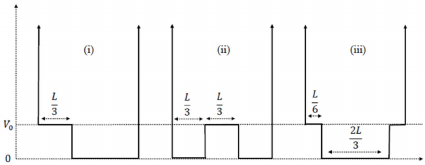
\includegraphics{figs/39.png}\end{figure}%[width=0.8\textwidth]{p25_diagram.png}
\end{center}
\begin{enumerate}
    \item $E_2 > E_1 > E_3$
    \item $E_3 > E_1 > E_2$
    \item $E_2 > E_3 > E_1$
    \item $E_3 > E_2 > E_1$
\end{enumerate}


\item
In cylindrical coordinates $(s, \phi, z)$, which of the following is a Hermitian operator?
\begin{enumerate}
    \item $\frac{1}{i} \frac{\partial}{\partial s}$
    \item $\frac{1}{i} \left( \frac{\partial}{\partial s} + \frac{1}{s} \right)$
    \item $\frac{1}{i} \left( \frac{\partial}{\partial s} + \frac{1}{2s} \right)$
    \item $\left( \frac{\partial}{\partial s} + \frac{1}{s} \right)$
\end{enumerate}


\item
A particle of mass 1 kg is released from a height of 1 m above the ground. When it reaches the ground, what is the value of Hamilton\textquotesingle s action for this motion in J s? ($g$ is the acceleration due to gravity; take gravitation potential to be zero on the ground)
\begin{enumerate}
    \item $-\frac{2}{3}\sqrt{2g}$
    \item $\frac{5}{3}\sqrt{2g}$
    \item $3\sqrt{2g}$
    \item $-\frac{1}{3}\sqrt{2g}$
\end{enumerate}


\item
If $(\dot{x}\dot{y} + \alpha xy)$ is a constant of motion of a two-dimensional isotropic harmonic oscillator with Lagrangian \begin{align*}L = \frac{m(\dot{x}^2 + \dot{y}^2)}{2} - \frac{k(x^2 + y^2)}{2}\end{align*} then $\alpha$ is
\begin{enumerate}
    \item $+\frac{k}{m}$
    \item $-\frac{k}{m}$
    \item $-\frac{2k}{m}$
    \item $0$
\end{enumerate}


\item
In a two-dimensional square lattice, frequency $\omega$ of phonons in the long wavelength limit changes linearly with the wave vector k. Then the density of states of phonons is proportional to
\begin{enumerate}
    \item $\omega$
    \item $\omega^2$
    \item $\sqrt{\omega}$
    \item $\frac{1}{\sqrt{\omega}}$
\end{enumerate}


\item
At T = 0 K, which of the following diagram represents the occupation probability $P(E)$ of energy states of electrons in a BCS type superconductor?
\begin{enumerate}
    \item \begin{figure}[H] \caption*{} \label{fig:44a}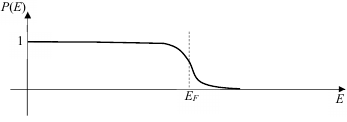
\includegraphics{figs/44a.png}\end{figure}%[width=0.4\textwidth]{p28_diagramA.png}
    \item \begin{figure}[H] \caption*{} \label{fig:44b}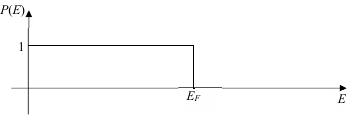
\includegraphics{figs/44b.png}\end{figure}%[width=0.4\textwidth]{p28_diagramB.png}
    \item \begin{figure}[H] \caption*{} \label{fig:44c}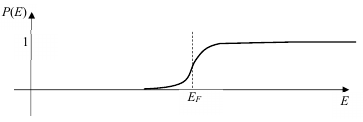
\includegraphics{figs/44c.png}\end{figure}%[width=0.4\textwidth]{p28_diagramC.png}
    \item \begin{figure}[H] \caption*{} \label{fig:44d}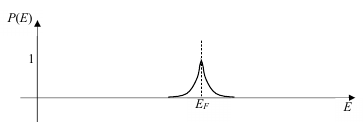
\includegraphics{figs/44d.png}\end{figure}%[width=0.4\textwidth]{p28_diagramD.png}
\end{enumerate}


\item
For a one-dimensional harmonic oscillator, the creation operator ($a^\dagger$) acting on the nth state $|\psi_n\rangle$, where $n = 0, 1, 2, \dots$, gives $a^\dagger|\psi_n\rangle = \sqrt{n + 1}|\psi_{n+1}\rangle$. The matrix representation of the position operator $x = \sqrt{\frac{\hbar}{2m\omega}}(a + a^\dagger)$ for the first three rows and columns is
\begin{enumerate}
    \item $\sqrt{\frac{\hbar}{2m\omega}} \myvec{ 1 & 0 & 0 \\ 0 & \sqrt{2} & 0 \\ 0 & 0 & \sqrt{3} }$
    \item $\sqrt{\frac{\hbar}{2m\omega}} \myvec{ 0 & 1 & 0 \\ 1 & 0 & 1 \\ 0 & 1 & 0 }$
    \item $\sqrt{\frac{\hbar}{2m\omega}} \myvec{ 0 & 1 & 0 \\ 1 & 0 & \sqrt{2} \\ 0 & \sqrt{2} & 0 }$
    \item $\sqrt{\frac{\hbar}{2m\omega}} \myvec{ 1 & 0 & \sqrt{3} \\ 0 & 0 & 0 \\ \sqrt{3} & 0 & 1 }$
\end{enumerate}


\item
A piston of mass m is fitted to an airtight horizontal cylindrical jar. The cylinder and piston have identical unit area of cross-section. The gas inside the jar has volume V and is held at pressure $P = P_{atmosphere}$. The piston is pushed inside the jar very slowly over a small distance. On releasing, the piston performs an undamped simple harmonic motion of low frequency. Assuming that the gas is ideal and no heat is exchanged with the atmosphere, the frequency of the small oscillations is proportional to
\begin{enumerate}
    \item $\sqrt{\frac{P\gamma}{mV}}$
    \item $\sqrt{\frac{P\gamma V}{m}}$
    \item $\sqrt{\frac{P}{mV^{\gamma-1}}}$
    \item $\sqrt{\frac{\gamma P}{mV^{\gamma-1}}}$
\end{enumerate}


\item
A paramagnetic salt of mass m is held at temperature T in a magnetic field H. If S is the entropy of the salt and M is its magnetization, then $dG = -SdT - MdH$, where G is the Gibbs free energy. If the magnetic field is changed adiabatically by $\Delta H \rightarrow 0$ and the corresponding infinitesimal changes in entropy and temperature are $\Delta S$ and $\Delta T$, then which of the following statements are correct
\begin{enumerate}
    \item $\Delta S = -\frac{1}{T} \left( \frac{\partial G}{\partial T} \right)_H \Delta T$
    \item $\Delta S = 0$
    \item $\Delta T = - \frac{\left( \frac{\partial M}{\partial T} \right)_H}{\left( \frac{\partial S}{\partial T} \right)_H} \Delta H$
    \item $\Delta T = 0$
\end{enumerate}


\item
A particle of mass m is moving inside a hollow spherical shell of radius $a$ so that the potential is
$V(r) = \begin{cases} 0 & \text{for } r < a \\ \infty & \text{for } r \ge a \end{cases}$
The ground state energy and wavefunction of the particle are $E_0$ and $R(r)$, respectively. Then which of the following options are correct?
\begin{enumerate}
    \item $E_0 = \frac{\hbar^2 \pi^2}{2ma^2}$
    \item $-\frac{\hbar^2}{2m} \frac{1}{r^2} \frac{d}{dr} \left( r^2 \frac{dR}{dr} \right) = E_0 R \quad (r < a)$
    \item $-\frac{\hbar^2}{2m} \frac{1}{r^2} \frac{d^2 R}{dr^2} = E_0 R \quad (r < a)$
    \item $R(r) = \frac{1}{r} \sin\left(\frac{\pi r}{a}\right) \quad (r < a)$
\end{enumerate}


\item
A particle of unit mass moves in a potential $V(r) = -V_0 e^{-r^2}$. If the angular momentum of the particle is $L = 0.5\sqrt{V_0}$, then which of the following statements are true?
\begin{enumerate}
    \item There are two equilibrium points along the radial coordinate
    \item There is one stable equilibrium point at $r_1$ and one unstable equilibrium point at $r_2 > r_1$
    \item There are two stable equilibrium points along the radial coordinate
    \item There is only one equilibrium point along the radial coordinate
\end{enumerate}


\item
In a diatomic molecule of mass $M$, electronic, rotational and vibrational energy scales are of magnitude $E_e$, $E_R$ and $E_V$, respectively. The spring constant for the vibrational energy is determined by $E_e$. If the electron mass is m then
\begin{enumerate}
    \item $E_R \sim \frac{m}{M} E_e$
    \item $E_R \sim \sqrt{\frac{m}{M}} E_e$
    \item $E_V \sim \sqrt{\frac{m}{M}} E_e$
    \item $E_V \sim \left(\frac{m}{M}\right)^{1/4} E_e$
\end{enumerate}


\item
Electronic specific heat of a solid at temperature $T$ is $C = \gamma T$, where $\gamma$ is a constant related to the thermal effective mass $(m_{eff})$ of the electrons. Then which of the following statements are correct?
\begin{enumerate}
    \item $\gamma \propto m_{eff}$
    \item $m_{eff}$ is greater than free electron mass for all solids
    \item Temperature dependence of $C$ depends on the dimensionality of the solid
    \item The linear temperature dependence of $C$ is observed at $T \ll$ Debye temperature
\end{enumerate}


\item
In a Hall effect experiment on an intrinsic semiconductor, which of the following statements are correct?
\begin{enumerate}
    \item Hall voltage is always zero
    \item Hall voltage is negative if the effective mass of holes is larger than those of electrons
    \item Hall coefficient can be used to estimate the carrier concentration in the semiconductor
    \item Hall voltage depends on the mobility of the carriers
\end{enumerate}


\item
A parallel plate capacitor with spacing $d$ and area of cross-section $A$ is connected to a source of voltage $V$. If the plates are pulled apart quasistatically to a spacing of $2d$, then which of the following statements are correct?
\begin{enumerate}
    \item The force between the plates at spacing $2d$ is $\frac{1}{8} \left( \frac{\epsilon_0 A V^2}{d^2} \right)$
    \item The work done in moving the plates is $\frac{1}{8} \left( \frac{\epsilon_0 A V^2}{d} \right)$
    \item The energy transferred to the voltage source is $\frac{1}{2} \left( \frac{\epsilon_0 A V^2}{d} \right)$
    \item The energy of the capacitor reduces by $\frac{1}{4} \left( \frac{\epsilon_0 A V^2}{d} \right)$
\end{enumerate}


\item
A system with time independent Hamiltonian $H(q, p)$ has two constants of motion $f(q, p)$ and $g(q, p)$. Then which of the following Poisson brackets are always zero?
\begin{enumerate}
    \item $\{H, f + g\}$
    \item $\{H, \{f, g\}\}$
    \item $\{H + f, g\}$
    \item $\{H, H + fg\}$
\end{enumerate}


\item
In the action-angle variables $(I_1, I_2, \theta_1, \theta_2)$, consider the Hamiltonian $H = 4I_1 I_2$ and $0 \le \theta_1, \theta_2 < 2\pi$. Let $\frac{I_1}{I_2} = \frac{1}{2}$. Which of the following are possible plots of the trajectories with different initial conditions in $\theta_1$-$\theta_2$ plane?
\begin{enumerate}
    \item \begin{figure}[H] \caption*{} \label{fig:55a}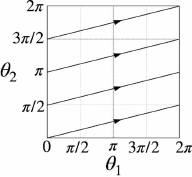
\includegraphics{figs/55a.png}\end{figure}%[width=0.4\textwidth]{p36_diagramA.png}
    \item \begin{figure}[H] \caption*{} \label{fig:55b}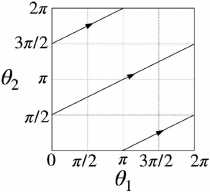
\includegraphics{figs/55b.png}\end{figure}%[width=0.4\textwidth]{p36_diagramB.png}
    \item \begin{figure}[H] \caption*{} \label{fig:55c}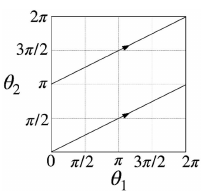
\includegraphics{figs/55c.png}\end{figure}%[width=0.4\textwidth]{p36_diagramC.png}
    \item \begin{figure}[H] \caption*{} \label{fig:55d}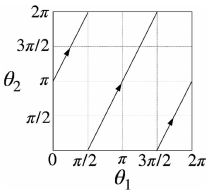
\includegraphics{figs/55d.png}\end{figure}%[width=0.4\textwidth]{p37_diagramD.png}
\end{enumerate}


\item
A particle of mass $m$ in the x-y plane is confined in an infinite two-dimensional well with vertices at (0, 0), (0, L), (L, L), (L, 0). The eigenfunctions of this particle are $\psi_{n_x, n_y} = \frac{2}{L} \sin\left(\frac{n_x \pi x}{L}\right) \sin\left(\frac{n_y \pi y}{L}\right)$. If perturbation of the form $V = Cxy$, where $C$ is a real constant, is applied, then which of the following statements are correct for the first excited state?
\begin{enumerate}
    \item The unperturbed energy is $\frac{3\pi^2\hbar^2}{2mL^2}$
    \item The unperturbed energy is $\frac{5\pi^2\hbar^2}{2mL^2}$
    \item First order energy shift due to the applied perturbation is zero
    \item The shift ($\delta$) in energy due to the applied perturbation is determined by an equation of the form $\mydet{ a - \delta & b \\ b & a - \delta } = 0$, where a and b are real, non-zero constants
\end{enumerate}


\item
A junction is formed between a metal on the left and an $n$-type semiconductor on the right. Before forming the junction, the Fermi level $E_F$ of the metal lies below that of the semiconductor. Then which of the following schematics are correct for the bands and the I-V characteristics of the junction?
\begin{enumerate}
    \item \begin{figure}[H] \caption*{} \label{fig:57a}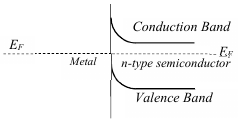
\includegraphics{figs/57a.png}\end{figure}%[width=0.6\textwidth]{p39_diagramA.png}
    \item \begin{figure}[H] \caption*{} \label{fig:57b}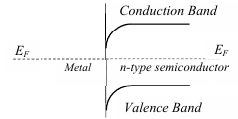
\includegraphics{figs/57b.png}\end{figure}%[width=0.6\textwidth]{p39_diagramB.png}
    \item \begin{figure}[H] \caption*{} \label{fig:57c}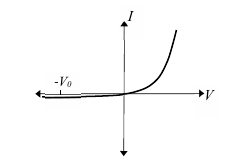
\includegraphics{figs/57c.png}\end{figure}%[width=0.6\textwidth]{p39_diagramC.png}
    \item \begin{figure}[H] \caption*{} \label{fig:57d}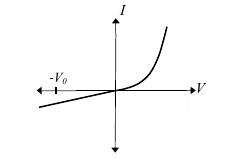
\includegraphics{figs/57d.png}\end{figure}%[width=0.6\textwidth]{p39_diagramD.png}
\end{enumerate}


\item
A plane polarized electromagnetic wave propagating in $y-z$ plane is incident at the interface of two media at Brewster\textquotesingle s angle. Taking $z = 0$ as the boundary between the two media, the electric field of the reflected wave is given by \begin{align*}\vec{E}_R = A_R \cos \left[ k_0 \left( \frac{\sqrt{3}}{2}y - \frac{1}{2}z \right) - \omega t \right] \hat{x}\end{align*} then which among the following statements are correct?
\begin{enumerate}
    \item The angle of refraction is $\frac{\pi}{6}$
    \item Ratio of permittivity of the medium of refraction ($\epsilon_2$) with respect to the medium on incidence ($\epsilon_1$), $\frac{\epsilon_2}{\epsilon_1} = 3$
    \item The incident wave can have components of its electric field in $y-z$ plane
    \item The angle of reflection is $\frac{\pi}{6}$
\end{enumerate}


\item
The minimum number of two-input NAND gates required to implement the following Boolean expression is \rule{1cm}{0.4pt}
\begin{align*}Y = [A\bar{B}(C + BD) + \bar{A}\bar{B}]C\end{align*}


\item
In a nucleus, the interaction $V_{so}\vec{l} \cdot \vec{s}$ is responsible for creating spin-orbit doublets. The energy difference between $p_{1/2}$ and $p_{3/2}$ states in units of $V_{so}\frac{\hbar^2}{2}$ is \rule{1cm}{0.4pt} (Round off to the nearest integer)


\item
Two identical particles of rest mass $m_0$ approach each other with equal and opposite velocity $v = 0.5c$, where $c$ is the speed of light. The total energy of one particle as measured in the rest frame of the other is $E = \alpha m_0 c^2$. The value of $\alpha$ is \rule{1cm}{0.4pt} (Round off to two decimal places)


\item
In an X-Ray diffraction experiment on a solid with FCC structure, five diffraction peaks corresponding to (111), (200), (220), (311) and (222) planes are observed using 1.54 \AA X-rays. On using 3 \AA X-rays on the same solid, the number of observed peaks will be \rule{1cm}{0.4pt}.

\item
For 1 mole of Nitrogen gas, the ratio $\brak{ \frac{\Delta S_{I}}{\Delta S_{II}} }$ of entropy change of the gas in processes (I) and (II) mentioned below is \rule{1cm}{0.4pt} (Round off to one decimal place)
(I) The gas is held at 1 atm and is cooled from 300 K to 77 K.
(II) The gas is liquified at 77 K.
(Take $C_p = 7.0$ cal mol$^{-1}$ K$^{-1}$, Latent heat $L = 1293.6$ cal mol$^{-1}$)


\item
Frequency bandwidth $\Delta\nu$ of a gas laser of frequency $\nu$ Hz is \begin{align*}\Delta\nu = \frac{2\nu}{c}\sqrt{\alpha A}\end{align*} where $\alpha = 3.44 \times 10^6$ m$^2$ s$^{-2}$ at room temperature and $A$ is the atomic mass of the lasing atom. For $^4$He - $^{20}$Ne laser (wavelength = 633 nm), $\Delta\nu = n \times 10^9$ Hz. The value of $n$ is \rule{1cm}{0.4pt} (Round off to one decimal place)


\item
A current of 1 A is flowing through a very long solenoid made of winding density 3000 turns/m. As shown in \figref{fig:65}, a parallel plate capacitor, with plates oriented parallel to the solenoid axis and carrying surface charge density $6\epsilon_0$ C m$^{-2}$, is placed at the middle of the solenoid. The momentum density of the electromagnetic field at the midpoint X of the capacitor is $n \times 10^{-13}$ N s m$^{-3}$. The value of $n$ is \rule{1cm}{0.4pt} (Round off to the nearest integer) (speed of light $c = 3 \times 10^8$ m s$^{-1}$)
    \begin{figure}[H] \centering \caption{} \label{fig:65}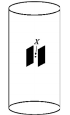
\includegraphics{figs/65.png}\end{figure}%[width=0.3\textwidth]{p42_diagram.png}


\end{enumerate}

\end{document}
